\documentclass[leqno,11pt]{article}
\usepackage{a4wide}
\usepackage[T1]{fontenc}
\usepackage[utf8]{inputenc}
\usepackage{graphicx}
\usepackage{amssymb}
\usepackage{amsthm}
\usepackage{url}
\usepackage{subfig}
%\textwidth 19cm
%\oddsidemargin -1.54cm

\setlength\parskip{0.13in}

\title{ocd - ocd c decompiler}
\date{\today}

\begin{document}

\newtheorem{definition}{Definition}
\maketitle

\tableofcontents

\newpage

\section{Introduction}

ocd is a C decompiler written in Python, currently supporting decompilation of programs compiled for the x64 architecture. The internal data structures used for instructions are quite universal, so it should be trivial to add additional architectures as they are needed, as well as new output languages. The decompiler performs some inferences as to the program structure (such as control and data flow analysis).

\section{Using ocd}

ocd reads a specified object file, performs decompilation on it and prints the results on standard output. It can also output a set of control flow graphs in dot format. 
\\ The usage of the program is as follows:

\begin{verbatim}
Usage: ocd.py [options] file

Options:
  -h, --help            show this help message and exit
  -d OPTION, --debug=OPTION
                        turn debug option on
  -g FILE, --graph=FILE
                        output a control flow graph
\end{verbatim}


An example control flow graph is shown in figure \ref{fig:cfg_example}.

\begin{figure}[h!]
\includegraphics[width=15cm]{images/cfg_example.eps}
\centering
\caption{A cfg example}
\label{fig:cfg_example}
\end{figure}

\section{Operation}

\subsection{Overview}

The decompilation occurs in stages. The program is built to be modular and each stage is separate. The stages are shown in figure \ref{fig:graph_stages}.

\begin{figure}[h!]
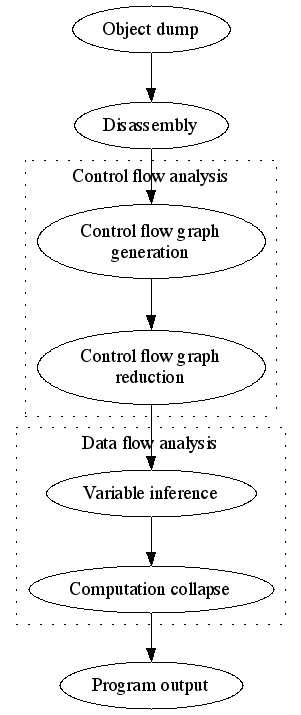
\includegraphics[height=10cm]{images/graph_stages.eps}
\centering
\caption{Stages of decompilation}
\label{fig:graph_stages}
\end{figure}

\subsection{Object dump}

Currently, ocd executes the GNU utility objdump and retrieves the list of object exports from it.

\subsection{Disassembly}

ocd supports decompilation of x86-64 and uses a modification of libdisassemble to disassemble code.

\subsection{Control flow analysis}

\subsubsection{Control flow graph generation}

\begin{definition}
A block of code is a list of instructions.
\end{definition}
\begin{definition}
$B_1$ is a subblock of $B_2$ if $B_1$ is a sublist of $B_2$.
\end{definition}
\begin{definition}
A block of code $B$ is uninterruptible if both of these conditions hold:
\begin{itemize}
 \item no instruction jumps to an instruction within $B$ other than the first (i.e. the only allowed entry point in $B$ is its head)
 \item no instruction in $B$, other than the last, jumps (i.e. the only exit point in $B$ is its last instruction)
\end{itemize}
\end{definition}
\begin{definition}
A block of code $B$ is maximally uninterruptible if it is interruptible and has both an entry point and an exit point.
\end{definition}
\begin{definition}
A control flow graph $cfg_B$ of a code block $B$ is a digraph $<V,E>$. The set of nodes $V$ is the set of all maximally uninterruptible subblocks of $B$. An edge $<B_1, B_2> \in E$ if and only if there is an instruction in $B_1$ that jumps to $B_2$.
\end{definition}

Generating the cfg of a block of code consists of finding all jumps in the block and then chopping the block into maximally interruptible blocks based on the list of jumps. An example cfg is given in figure \ref{fig:cfg_example}.

\subsubsection{Control flow graph reduction}

A cfg of a block of code gives insight into how control flows through the block of code and ideally gives insight into what the program structure was originally. 

\begin{figure}[h!]
  \centering
  \subfloat[if]{\label{fig:cfg_if}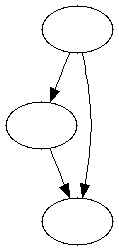
\includegraphics[height=4cm]{images/cfg_if}}
  \hspace{1cm}             
  \subfloat[if/else]{\label{fig:cfg_ifelse}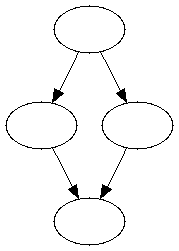
\includegraphics[height=4cm]{images/cfg_ifelse}}
  \hspace{1cm}             
  \subfloat[while]{\label{fig:cfg_while}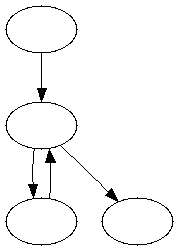
\includegraphics[height=4cm]{images/cfg_while}}
  \hspace{1cm}             
  \subfloat[pass]{\label{fig:cfg_cons}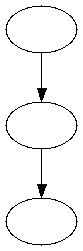
\includegraphics[height=4cm]{images/cfg_cons}}
  \caption{Cfg patterns}
  \label{fig:cfg_patterns}
\end{figure}

Logical structures can be recognized by finding patterns in the cfg. The patterns are listed in figure \ref{fig:cfg_patterns}. The patterns are used to define a decreasing graph rewriting system (not unlike a context-sensitive grammar) in which a single step finds a pattern and contracts it to a single node containing information about the pattern's respective logical structure. Ideally, the fixed point of such a transformation will result in a single node containing the abstract syntax tree of the original program.

\subsection{Data flow analysis}

\subsubsection{Variable inference}

In this phase, instruction operands are substituted with newly assigned names.

\subsection{Computation collapse}

In this phase, the program's computation is analyzed. Dead instructions are removed and others are folded into more coherent expressions. For example,

\begin{verbatim}
a = a + 1
b = a * 2
n = 2
n = b - a
\end{verbatim}

might be converted into:

\begin{verbatim}
n = (a+1)*2-a+1
\end{verbatim}

\subsection{Program output}

The program is output recursively on the cfgs of its symbols.

\section{Contributing to ocd}

ocd uses git as its SCM. The master repository is hosted at \url{http://github.com/drx/ocd}. If you want to contribute to the project, you can ask the current maintainer to add you to the contributors list. Alternatively, you can fork the project and then request that your changes be merged to the original project.

\section{Copyright}

\begin{verbatim}
 Copyright (c) 2010 Alek Balicki, Łukasz Zapart

 Permission is hereby granted, free of charge, to any person
 obtaining a copy of this software and associated documentation
 files (the "Software"), to deal in the Software without
 restriction, including without limitation the rights to use,
 copy, modify, merge, publish, distribute, sublicense, and/or sell
 copies of the Software, and to permit persons to whom the
 Software is furnished to do so, subject to the following
 conditions:

 The above copyright notice and this permission notice shall be
 included in all copies or substantial portions of the Software.

 THE SOFTWARE IS PROVIDED "AS IS", WITHOUT WARRANTY OF ANY KIND,
 EXPRESS OR IMPLIED, INCLUDING BUT NOT LIMITED TO THE WARRANTIES
 OF MERCHANTABILITY, FITNESS FOR A PARTICULAR PURPOSE AND
 NONINFRINGEMENT. IN NO EVENT SHALL THE AUTHORS OR COPYRIGHT
 HOLDERS BE LIABLE FOR ANY CLAIM, DAMAGES OR OTHER LIABILITY,
 WHETHER IN AN ACTION OF CONTRACT, TORT OR OTHERWISE, ARISING
 FROM, OUT OF OR IN CONNECTION WITH THE SOFTWARE OR THE USE OR
 OTHER DEALINGS IN THE SOFTWARE.
\end{verbatim}


\end{document}
